\begin{question}
%\begin{instance}  
%\begin{statement}
%\framebox{\begin{minipage}{0.99\textwidth}\vspace*{5pt}	
%{\fontsize{18}{22}\selectfont  
%Lee el siguiente texto:\par
%
%¡Hola Ali!\par
%
%Te escribo sobre mi escritor favorito: Gabriel García Márquez. Él fue un escritor  y periodista colombiano muy famoso en Latinoamérica y en todo el mundo. Nació en 1927 y cuando estudiaba en la escuela secundaria escribía poesía. Estudió en la universidad en Bogotá, la capital de Colombia. Cuando era pequeño no le gustaban los deportes, pero en la universidad practicó deportes como fútbol y béisbol. Gabriel trabajó como periodista con varios periódicos en diferentes ciudades de Colombia. Para Gabriel la política era muy importante. Sin embargo, la mayoría de sus trabajos fueron novelas y cuentos cortos. Sus novelas más famosas se llaman “Cien Años de Soledad” y “El Amor en los Tiempos del Cólera”. En sus historias, Gabriel combinaba la realidad y la fantasía. En 1982 Gabriel ganó el Premio Nobel de Literatura por su fantástico trabajo. Murió en 2014 pero la gente todavía lee sus libros en todo el mundo.\par
%¿Y tú? ¿Quién es tu escritor favorito?\par
%Un abrazo,\par
%Juan\par}
%\vspace*{5pt}\end{minipage}}  
%\end{statement}\vspace*{40pt}
%\end{instance}
\begin{center}
	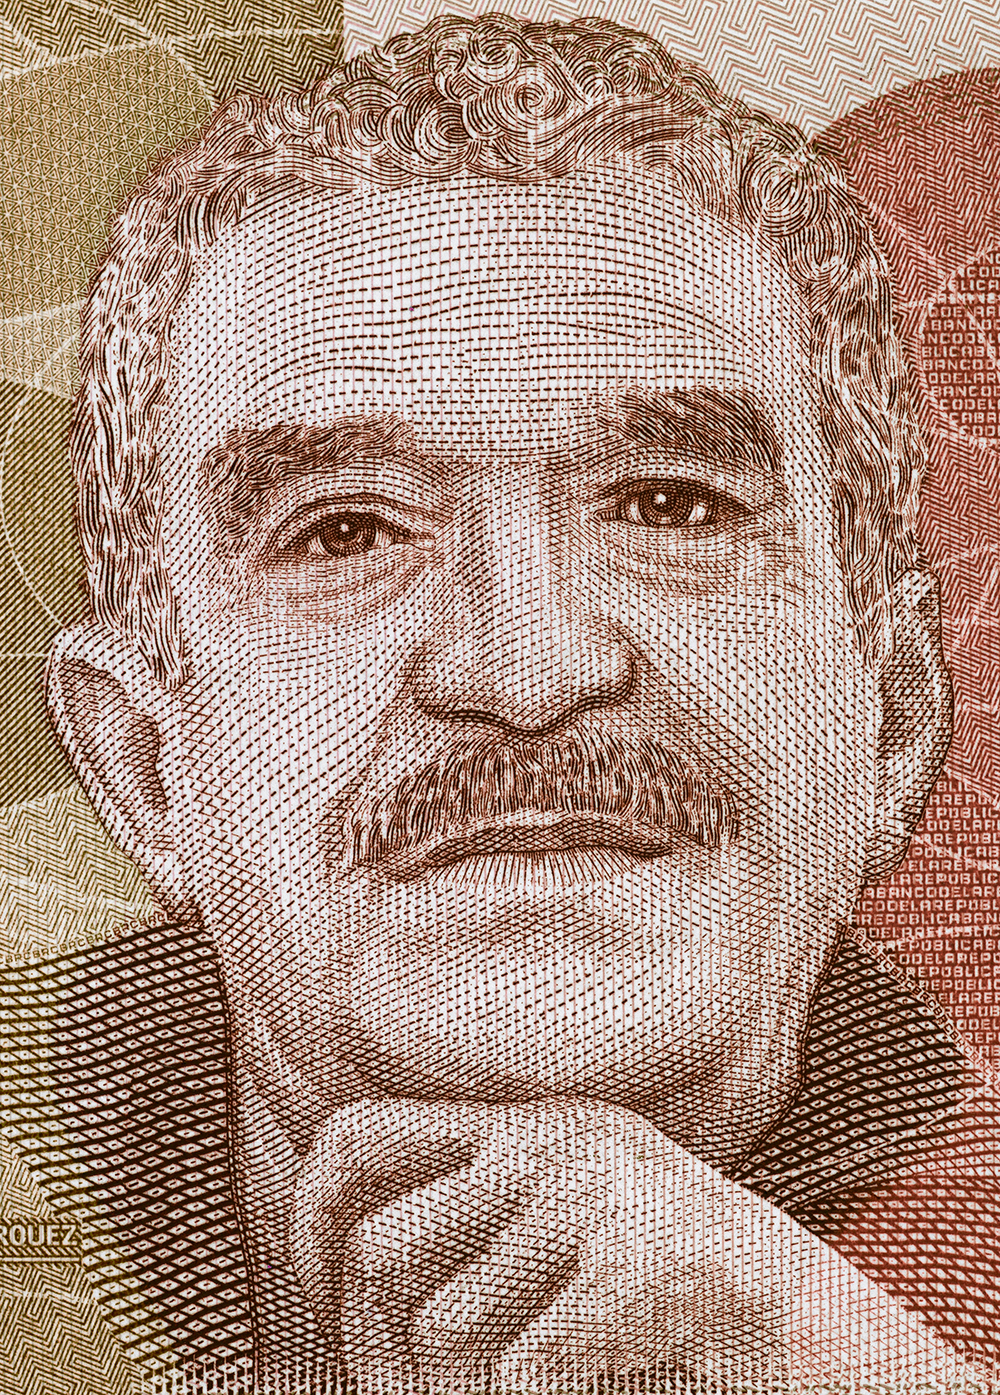
\includegraphics[width=0.45\textwidth]{308167846093.jpg}
\end{center}
\end{question}
